\documentclass[4paper]{article}
\usepackage[spanish]{babel}
%\usepackage[ansinew]{inputenc}
\usepackage[utf8x]{inputenc}
%\usepackage[utf-8]{inputenc}
%\usepackage[T1]{fontenc}
\usepackage{graphicx}
\usepackage{multicol}
\usepackage{float}
%\usepackage{longtable}
%\usepackage{array}
%\usepackage{multirow}
%\usepackage[latin1]{inputenc}
%\inputencoding{latin1}

\renewcommand{\tablename}{Tabla}
\renewcommand{\S}{Sqlite }
\author{Manuel Molino Milla \and Luis Molina Garzón}
\title{\textbf{\S}}
\date{\today}

\begin{document}
\maketitle 
\tableofcontents
\newpage

\section{Características}
\begin{itemize}
\item Es un sistema de gestión de bases de datos relacional contenida en una relativamente pequeña (menos de 500 kB) biblioteca escrita en C. 
\item Es un proyecto de dominio público creado por D. Richard Hipp de uso para cualquier proposito.
\item A diferencia de los sistema de gestión de bases de datos cliente-servidor, el motor de SQLite NO es un proceso independiente con el que el programa principal se comunica. 
\item  El conjunto de la base de datos (definiciones, tablas, índices, y los propios datos), son guardados como un sólo fichero estándar en la máquina host. 
\item Este diseño simple se logra bloqueando todo el fichero de base de datos al principio de cada transacción.
\item En su versión 3, SQLite permite bases de datos de hasta 140 Terabytes de tamaño, y también permite la inclusión de campos tipo BLOB.
\end{itemize}
Recomendaciones:\\
Tal y com comenta la página oficial son muchos los usos de recomendación, pero llama la atención las siguientes apreciaciones:
\begin{itemize}
\item Si los datos están separados de la aplicación por red, \emph{recomendado uso de una tecnología cliente/servidor}
\item En el caso de alta concurrencia de escritura de datos, \emph{recomendado uso de una tecnología cliente/servidor}
\item Para \emph{big/data}, \emph{recomendado uso de una tecnología cliente/servidor}
\item Para el RESTO \emph{elige SQLite}
\end{itemize}
Ejemplo de usos:
\begin{itemize}
\item Para aplicaciones embebidas en dispositivos (TV, consolas, cámaras, sensores remotos, drones, \dots)
\item Aplicaciones de escritorio.
\item \emph{Websites} En términos generales , cualquier sitio que recibe menos de 100K visitas / día debería funcionar bien con SQLite \textbf{(sic)}
\item Análisis de datos (usando shell sqlite o lenguajes como python o R).
\item Caché de datos (Firefox).
\item \dots
\end{itemize}

\section{Tipo de datos}
Desde la versión 3 SQLite usa un tipado mas o menos dinámico, es decir el tipo va a depender del literal y no del valor declarado en el esquema. 
\begin{enumerate}
\item[NULL] para valores nulo.
\item[INTEGER] para valores enteros.
\item[REAL] para números en coma flotante usando el estándar 8-byte IEEE
\item[TEXT] para texto.
\item[BLOB] para valores binarios.
\end{enumerate}
Para facilitar la compatibilidad entre SQLite y otras bases de datos, soporta el concepto de afinidad, de manera que podamos definir otro tipo de datos, ejemplo podemos definir un \emph{TINYINT} que se almacenará como \emph{INTEGER}, o e caso de un VARCHAR(255) que se almacena como \emph{TEXT} o el caso de \emph{BOOLEAN} que se almacena como \emph{NUMERIC}. En el caso de \emph{NUMERIC} implica que se convierten los datos bien a \emph{INTEGER} o \emph{REAL}, puede pasar para datos de tipo \emph{DATE} o \emph{DATETIME}
\begin{figure}[H]
\centering
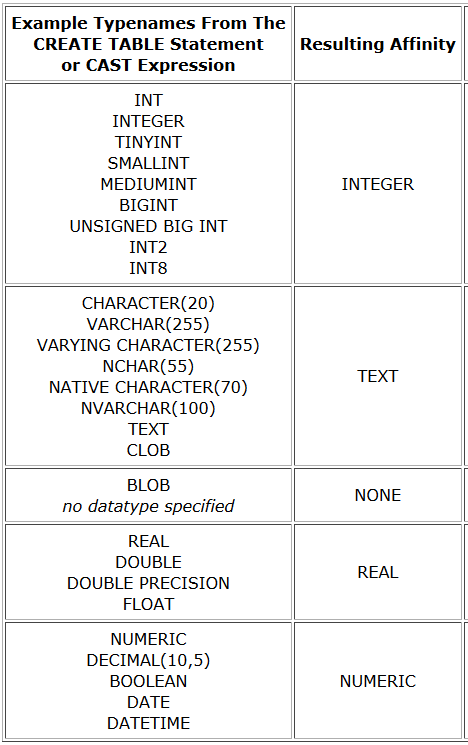
\includegraphics[scale=0.5]{afinidad.png}
\end{figure}

\section{Instalación}
Descargamos la aplicación desde \emph{http://www.sqlite.org/download.html} y elegimos la opción que sea de nuestro gusto.\par
Posteriormente descomprimimos con \emph{unzip}, se crea un nuevo directorio que contiene el ejecutable y ejecutamos con \emph{./sqlite3}:
\begin{verbatim}
usuario@portatil:~/sqlite/sqlite-tools-linux-x86-3120200$ ./sqlite3
SQLite version 3.12.2 2016-04-18 17:30:31
Enter ".help" for usage hints.
Connected to a transient in-memory database.
Use ".open FILENAME" to reopen on a persistent database.
sqlite>
\end{verbatim}

\section{Ejemplo}
Vamos a utilizar una BD con el siguiente esquema:\\
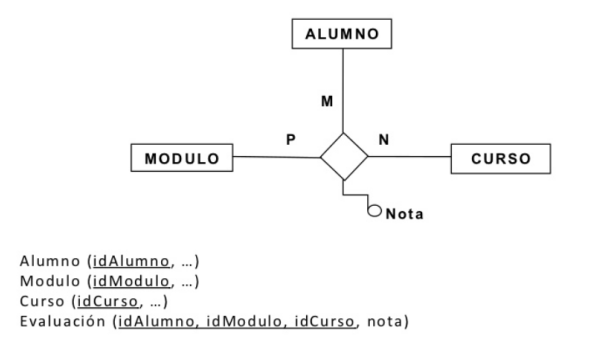
\includegraphics[scale=0.5]{ejemplo.png}

\section{Creacion de la BD}
Para la creación de la BD solo hace falta ejecutar \emph{./sqlite3 ejemplo} donde ejemplo será el nombre de la BD. El resultado de la ejución es una terminal preparada para establecer el esquema de dicha BD.
\begin{verbatim}
usuario@portatil:~/sqlite/sqlite-tools-linux-x86-3120200$ ./sqlite3 ejemplo
SQLite version 3.12.2 2016-04-18 17:30:31
Enter ".help" for usage hints.
sqlite>
\end{verbatim}

\section{Establecimiento de soporte de integridad referencial}
Por defecto \S no permite \emph{foreign keys} para ello hay que forzar el su uso:
\begin{verbatim}
usuario@portatil:~/sqlite/sqlite-tools-linux-x86-3120200$ ./sqlite3 ejemplo
SQLite version 3.12.2 2016-04-18 17:30:31
Enter ".help" for usage hints.
sqlite> PRAGMA foreign_keys;
0
sqlite> PRAGMA foreign_keys = ON;
sqlite> PRAGMA foreign_keys;
1
\end{verbatim} 

\section{Creacion de las tablas}
Vamos a usar el siguiente esquema:
\begin{verbatim}
PRAGMA foreign_keys = ON;

DROP TABLE IF EXISTS alumno;
CREATE TABLE alumno (
        id INTEGER PRIMARY KEY AUTOINCREMENT,
        nombre TEXT,
        apellidos TEXT
);

DROP TABLE IF EXISTS modulo;
CREATE TABLE modulo (
        id INTEGER PRIMARY KEY AUTOINCREMENT,
        nombre TEXT,
        numeroHoras INTEGER
);

DROP TABLE IF EXISTS curso;
CREATE TABLE curso (
        id INTEGER PRIMARY KEY AUTOINCREMENT,
        nombre TEXT,
        aula TEXT
);

DROP TABLE IF EXISTS evaluacion;
CREATE TABLE evaluacion (
        idAlumno INTEGER,
        idModulo INTEGER,
        idCurso INTEGER,
        notas INTEGER,
        PRIMARY KEY(idAlumno,idModulo,idCurso),
        FOREIGN KEY(idAlumno) REFERENCES alumno(id) ON DELETE CASCADE,
        FOREIGN KEY(idModulo) REFERENCES modulo(id) ON DELETE CASCADE,
        FOREIGN KEY(idCurso) REFERENCES curso(id) ON DELETE CASCADE
);
\end{verbatim}
Para cargarla usamos el comando \emph{read} que permite ejecutar sentencias SQL desde un fichero:
\begin{verbatim}
sqlite> .read crear_tablas.sql
\end{verbatim}


\section{Indices en las tablas}
El índice de una base de datos es una estructura de datos que mejora la velocidad de las operaciones mediante un identificador único de cada fila de una tabla, permitiendo un rápido acceso a los registros de una tabla en una base de datos. Al aumentar drásticamente la velocidad de acceso, se suelen usar, sobre aquellos campos sobre los cuales se hacen frecuentes búsquedas.\par
El índice tiene un funcionamiento similar al índice de un libro, guardando parejas de elementos: el elemento que se desea indexar y su posición en la base de datos.\par
Los índices pueden ser creados usando una o más columnas, proporcionando la base tanto para búsquedas rápidas al azar como de un ordenado acceso a registros eficiente.\par
Para la creación en \S podemos hacer\par
\begin{quote}
CREATE INDEX apell ON alumno(apellidos);
\end{quote}
\section{Insertar datos}
Podemos hacerlo desde un fichero usando de nuevo el comando \emph{.read}. Vamos a importar los siguientes datos:
\begin{verbatim}
INSERT INTO alumno (nombre,apellidos) VALUES ("Juan", "García Paniagua");
INSERT INTO alumno (nombre,apellidos) VALUES ("Pedro", "Buendía García");
INSERT INTO alumno (nombre,apellidos) VALUES ("Jacinto", "Piedra Hita");
INSERT INTO alumno (nombre,apellidos) VALUES ("Pedro", "Nuñez García");
INSERT INTO alumno (nombre,apellidos) VALUES ("Inmaculada", "Beñat Polonia");
INSERT INTO alumno (nombre,apellidos) VALUES ("Rocío", "Cornejo García");
INSERT INTO alumno (nombre,apellidos) VALUES ("Victoria", "Buendía Benito");
INSERT INTO alumno (nombre,apellidos) VALUES ("Mª Dolores", "Molinos Codoba");
INSERT INTO alumno (nombre,apellidos) VALUES ("Alejandro ", "Zapatero Aznar");
INSERT INTO alumno (nombre,apellidos) VALUES ("Ángel", "Gómez Gómez");
INSERT INTO alumno (nombre,apellidos) VALUES ("Luisa", "Peralez Santiago");
INSERT INTO alumno (nombre,apellidos) VALUES ("Felix", "Barou García-Concha");
INSERT INTO alumno (nombre,apellidos) VALUES ("Samuel", "García Fernández");



INSERT INTO modulo (nombre,numeroHoras) VALUES ("Base de datos", 8);
INSERT INTO modulo (nombre,numeroHoras) VALUES ("Programación", 8);
INSERT INTO modulo (nombre,numeroHoras) VALUES ("Lenguajes de marcas", 4);

INSERT INTO curso (nombre, aula) VALUES ("Segundo A", "Aula 1");
INSERT INTO curso (nombre, aula) VALUES ("Segundo B", "Aula 2");

INSERT INTO evaluacion VALUES (1,1,1,5);
INSERT INTO evaluacion VALUES (1,2,1,6);
INSERT INTO evaluacion VALUES (1,3,1,4);
INSERT INTO evaluacion VALUES (2,1,1,4);
INSERT INTO evaluacion VALUES (2,2,1,5);
INSERT INTO evaluacion VALUES (2,3,1,6);
INSERT INTO evaluacion VALUES (3,1,1,6);
INSERT INTO evaluacion VALUES (3,2,1,1);
INSERT INTO evaluacion VALUES (3,3,1,10);
INSERT INTO evaluacion VALUES (4,1,1,5);
INSERT INTO evaluacion VALUES (4,2,1,6);
INSERT INTO evaluacion VALUES (4,3,1,1);
INSERT INTO evaluacion VALUES (5,1,1,6);
INSERT INTO evaluacion VALUES (5,2,1,6);
INSERT INTO evaluacion VALUES (5,3,1,6);
INSERT INTO evaluacion VALUES (6,1,1,2);
INSERT INTO evaluacion VALUES (6,2,1,8);
INSERT INTO evaluacion VALUES (6,3,1,7);
INSERT INTO evaluacion VALUES (7,1,1,6);
INSERT INTO evaluacion VALUES (7,2,1,6);
INSERT INTO evaluacion VALUES (7,3,1,6);
INSERT INTO evaluacion VALUES (8,1,1,3);
INSERT INTO evaluacion VALUES (8,2,1,0);
INSERT INTO evaluacion VALUES (8,3,1,1);
INSERT INTO evaluacion VALUES (9,1,2,6);
INSERT INTO evaluacion VALUES (9,2,2,6);
INSERT INTO evaluacion VALUES (9,3,2,6);
INSERT INTO evaluacion VALUES (10,1,2,1);
INSERT INTO evaluacion VALUES (10,2,2,1);
INSERT INTO evaluacion VALUES (10,3,2,1);
INSERT INTO evaluacion VALUES (11,1,2,6);
INSERT INTO evaluacion VALUES (11,2,2,8);
INSERT INTO evaluacion VALUES (11,3,2,9);
INSERT INTO evaluacion VALUES (12,1,2,9);
INSERT INTO evaluacion VALUES (12,2,2,10);
INSERT INTO evaluacion VALUES (12,3,2,3);
INSERT INTO evaluacion VALUES (13,1,2,3);
INSERT INTO evaluacion VALUES (13,2,2,3);
INSERT INTO evaluacion VALUES (13,3,2,4);
\end{verbatim}
Y esto nos dará después de la importación:
\begin{verbatim}
sqlite> select * from alumno;
1|Juan|García Paniagua
2|Pedro|Buendía García
3|Jacinto|Piedra Hita
4|Pedro|Nuñez García
5|Inmaculada|Beñat Polonia
6|Rocío|Cornejo García
7|Victoria|Buendía Benito
8|Mª Dolores|Molinos Codoba
9|Alejandro |Zapatero Aznar
10|Ángel|Gómez Gómez
11|Luisa|Peralez Santiago
12|Felix|Barou García-Concha
13|Samuel|García Fernández
\end{verbatim}
Podemos cambiar la forma de imprimirlo con \emph{.mode}
\begin{verbatim}
.mode MODE ?TABLE?     Set output mode where MODE is one of:
                         csv      Comma-separated values
                         column   Left-aligned columns.  (See .width)
                         html     HTML <table> code
                         insert   SQL insert statements for TABLE
                         line     One value per line
                         list     Values delimited by .separator string
                         tabs     Tab-separated values
                         tcl      TCL list elements
\end{verbatim}
Cambiando a \emph{.mode tabs} tendremos resultado como:
\begin{verbatim}
sqlite> select * from modulo;
1	Base de datos	8
2	Programación	8
3	Lenguajes de marcas	4
\end{verbatim}
\section{Ejemplo de consultas}
\begin{verbatim}
sqlite> .separator "<==>"     
sqlite> .mode list
sqlite> select notas, alumno.nombre, alumno.apellidos, modulo.nombre from \
alumno, modulo, evaluacion, curso where alumno.id=evaluacion.idAlumno and \
modulo.id=idModulo and curso.id=1;
\end{verbatim}
Que origina la siguiente consulta:
\begin{verbatim}
5<==>Juan<==>García Paniagua<==>Base de datos
6<==>Juan<==>García Paniagua<==>Programación
4<==>Juan<==>García Paniagua<==>Lenguajes de marcas
4<==>Pedro<==>Buendía García<==>Base de datos
5<==>Pedro<==>Buendía García<==>Programación
6<==>Pedro<==>Buendía García<==>Lenguajes de marcas
6<==>Jacinto<==>Piedra Hita<==>Base de datos
1<==>Jacinto<==>Piedra Hita<==>Programación
10<==>Jacinto<==>Piedra Hita<==>Lenguajes de marcas
5<==>Pedro<==>Nuñez García<==>Base de datos
6<==>Pedro<==>Nuñez García<==>Programación
1<==>Pedro<==>Nuñez García<==>Lenguajes de marcas
6<==>Inmaculada<==>Beñat Polonia<==>Base de datos
6<==>Inmaculada<==>Beñat Polonia<==>Programación
6<==>Inmaculada<==>Beñat Polonia<==>Lenguajes de marcas
2<==>Rocío<==>Cornejo García<==>Base de datos
8<==>Rocío<==>Cornejo García<==>Programación
7<==>Rocío<==>Cornejo García<==>Lenguajes de marcas
6<==>Victoria<==>Buendía Benito<==>Base de datos
6<==>Victoria<==>Buendía Benito<==>Programación
6<==>Victoria<==>Buendía Benito<==>Lenguajes de marcas
3<==>Mª Dolores<==>Molinos Codoba<==>Base de datos
0<==>Mª Dolores<==>Molinos Codoba<==>Programación
1<==>Mª Dolores<==>Molinos Codoba<==>Lenguajes de marcas
6<==>Alejandro <==>Zapatero Aznar<==>Base de datos
6<==>Alejandro <==>Zapatero Aznar<==>Programación
6<==>Alejandro <==>Zapatero Aznar<==>Lenguajes de marcas
1<==>Ángel<==>Gómez Gómez<==>Base de datos
1<==>Ángel<==>Gómez Gómez<==>Programación
1<==>Ángel<==>Gómez Gómez<==>Lenguajes de marcas
6<==>Luisa<==>Peralez Santiago<==>Base de datos
8<==>Luisa<==>Peralez Santiago<==>Programación
9<==>Luisa<==>Peralez Santiago<==>Lenguajes de marcas
9<==>Felix<==>Barou García-Concha<==>Base de datos
10<==>Felix<==>Barou García-Concha<==>Programación
3<==>Felix<==>Barou García-Concha<==>Lenguajes de marcas
3<==>Samuel<==>García Fernández<==>Base de datos
3<==>Samuel<==>García Fernández<==>Programación
4<==>Samuel<==>García Fernández<==>Lenguajes de marcas
\end{verbatim}

\section{Vistas en \S}
Una vista no es mas que una sentencia \emph{SQL} que se almacena en la BD con un nombre asociado. Por lo tanto almacena los datos de una tabla, o parte de un tabla en función del tipo de consulta, o bien de varias tablas en el caso de hacer \emph{subconsultas} o \emph{join}\par
Ejemplo una cosulta puede ser nombre y apellidos de los alumnos que pertenecen a \emph{Segundo A} con sus notas del módulo Base de datos:
\begin{quote}
select alumno.nombre, alumno.apellidos, evaluacion.notas from alumno, curso, modulo, evaluacion where alumno.id=evaluacion.idAlumno and curso.id=evaluacion.idCurso and modulo.id=evaluacion.idModulo and modulo.nombre='Base de datos' and curso.nombre='Segundo A';
\end{quote}
Que nos dá:
\begin{verbatim}
Juan|García Paniagua|5
Pedro|Buendía García|4
Jacinto|Piedra Hita|6
Pedro|Nuñez García|5
Inmaculada|Beñat Polonia|6
Rocío|Cornejo García|2
Victoria|Buendía Benito|6
Mª Dolores|Molinos Codoba|3
\end{verbatim}
La vista se crea con el comando CREATE VIEW \emph{nombreVista} AS \emph{sentencia}
Ejemplo anterior:
\begin{quote}
CREATE VIEW bd\_2A AS select alumno.nombre, alumno.apellidos, evaluacion.notas from alumno, curso, modulo, evaluacion where alumno.id=evaluacion.idAlumno and curso.id=evaluacion.idCurso and modulo.id=evaluacion.idModulo and modulo.nombre='Base de datos' and curso.nombre='Segundo A';
\end{quote}
La consulta anterios es igual a hacer:
\begin{quote}
select * from bd\_2a;
\end{quote}
También se pueden haces consultas sobre dicha vista, por ejemplo de los datos anteriores queremos los alumnos que aprueban:
\begin{quote}
select * from bd\_2a where notas$>=$5;
\end{quote}
Cuya salida es:
\begin{verbatim}
Juan|García Paniagua|5
Jacinto|Piedra Hita|6
Pedro|Nuñez García|5
Inmaculada|Beñat Polonia|6
Victoria|Buendía Benito|6
\end{verbatim}

\section{Triggers}
Un trigger (o disparador) en una Base de datos, es un procedimiento que se ejecuta cuando se cumple una condición establecida al realizar una operación. Dependiendo de la base de datos, los triggers pueden ser de inserción (INSERT), actualización (UPDATE) o borrado (DELETE). Algunas bases de datos pueden ejecutar triggers al crear, borrar o editar usuarios, tablas, bases de datos u otros objetos.\par 
El escenario del ejemplo es el siguiente, cuando un alumno se de de baja se creará una tupla con los datos del alumno y la fecha de baja en una tabla historial, pare esto se puede usar el siguiente esquema que crea la tabla y el\emph{trigger}:
\begin{verbatim}
DROP TABLE IF EXISTS historial;
CREATE TABLE historial (
        id INTEGER PRIMARY KEY AUTOINCREMENT,
        nombre TEXT,
        apellidos TEXT,
        fecha_baja TEXT
);

DROP TRIGGER IF EXISTS borrado;
CREATE TRIGGER borrado BEFORE DELETE
ON alumno
BEGIN
        INSERT INTO historial (nombre, apellidos, fecha_baja) VALUES
        (old.nombre, old.apellidos, datetime('now'));
END;
\end{verbatim}

\section{Esquema final de la BD}
Al final la BD queda, tras ejecutar el comando \emph{.sqlite}:
\begin{verbatim}
sqlite> .schema
CREATE TABLE alumno (
        id INTEGER PRIMARY KEY AUTOINCREMENT,
        nombre TEXT,
        apellidos TEXT
);
CREATE TABLE modulo (
        id INTEGER PRIMARY KEY AUTOINCREMENT,
        nombre TEXT,
        numeroHoras INTEGER
);
CREATE TABLE curso (
        id INTEGER PRIMARY KEY AUTOINCREMENT,
        nombre TEXT,
        aula TEXT
);
CREATE TABLE evaluacion (
        idAlumno INTEGER,
        idModulo INTEGER,
        idCurso INTEGER,
        notas INTEGER,
        PRIMARY KEY(idAlumno,idModulo,idCurso),
        FOREIGN KEY(idAlumno) REFERENCES alumno(id) ON DELETE CASCADE,
        FOREIGN KEY(idModulo) REFERENCES modulo(id) ON DELETE CASCADE,
        FOREIGN KEY(idCurso) REFERENCES curso(id) ON DELETE CASCADE
);
CREATE INDEX apell ON alumno(apellidos);
CREATE VIEW bd_2A AS select alumno.nombre, alumno.apellidos, evaluacion.notas from alumno,
 curso, modulo, evaluacion where alumno.id=evaluacion.idAlumno and 
 curso.id=evaluacion.idCurso  and modulo.id=evaluacion.idModulo and
 modulo.nombre="Base de datos" and curso.nombre='Segundo A';
CREATE TABLE historial (
        id INTEGER PRIMARY KEY AUTOINCREMENT,
        nombre TEXT,
        apellidos TEXT,
	fecha_baja TEXT
);
CREATE TRIGGER borrado BEFORE DELETE
ON alumno
BEGIN
	INSERT INTO historial (nombre, apellidos, fecha_baja) 
	VALUES (old.nombre, old.apellidos, datetime('now'));
END;
\end{verbatim}
\section{Copia de seguridad}
Se puede hacer una copia con el comando \emph{.backup}\par 
También se puede tratar como una copia de seguridad de un fichero de sistema.

\section{Ejercicio final}
El ejercicio final consiste en la realizacion de una BD para inventariar libros y permitir su posterior prestamo. Para esto hay que tener en cuenta los siguientes datos:
\begin{itemize}
\item Los libros pueden pertenecer a una única categoria, que puede ser: Bases de datos, programacion, redes, ofimatica, hardware, seguridad, aplicaciones web,  sistemas operativos o miscelanea.
\item De los libros debemos conocer el nombre, autor y editorial.
\item De los usuarios su nombre y apellidos.
\item Los libros pueden ser prestados, lo unico que tenemos que conocer es la persona que lo retira y la fecha de prestamo. 
\item Prepara las siguientes consultas, si es necesario prepara vistas para las mismas.
\begin{enumerate}
\item El numero de libros prestados.
\item El listado de libros prestados.
\item El listado de libros por categorias.
\item El listado de libros prestados por categorias.
\item El listado de libros no prestados por categorias.
\item El listado de libros no prestados.
\item Los libros prestados a un usuario.
\item Listado de usuarios.
\end{enumerate}
\item Prepara dos triggers para dar de baja a usuarios y libros.
\end{itemize}
\end{document}
